First, we provide a pre-processing step with the objective of having a segmented point set of the object \ref{sec:pre}. This is then used to create the probabilistic shape representation \ref{sec:object}. This is then exploited in 

%%%%%%%%%%%%%%%%%%%%%%%%%%%%%%%%%%%%%%%%
\subsection{Object Segmentation}
\label{sec:segmentation}

\citep[Sec.~III.A]{Hudson2012Endtoend} provides good candidates for object segmentation that are well oriented to object grasp, manipulation, and for our purposes, exploration. In fact, the combination of their ``Table Plane Estimation'' with their ``Volume-Based Segmentation'' yields the ubiquituos tabletop object segmentation \citep{TabletopObjectDetector}. However, to improve the rechability of the exploration, we prefer to hold the object in one hand-arm system and explore with another, as described in Sec.~\ref{sec:scope}. Thus, our selected approach for object segmentation is simpler than those approaches. The difficulties is in measuring the configuration of a soft and adaptable gripper that keeps the object in position to filter out the points belonging to the hand-arm system. For this purpose, one can rely in body-type measurements instead of traditional encoders, as described by~\citet{Santaera2015Lowcost}. Once the hand-arm system pose is measured, then a trivial passthrough filter with slightly scaled bounding boxes of the robot geometry is used to obtain a point cloud of the object isolated from the scene. Algorithm~\ref{alg:in-hand-segmentation} shows the pseudo-code of this procedure, indicating the actual. Additionally, 

It is worth noting, that this module is here just to show how visual and tactile data might be merged into a single shape model. But as a matter of fact, the initial training point set can be empty and start by simply probing naively towards the gripper to initialize the training set.

\begin{figure}
\centering
  \mbox{
  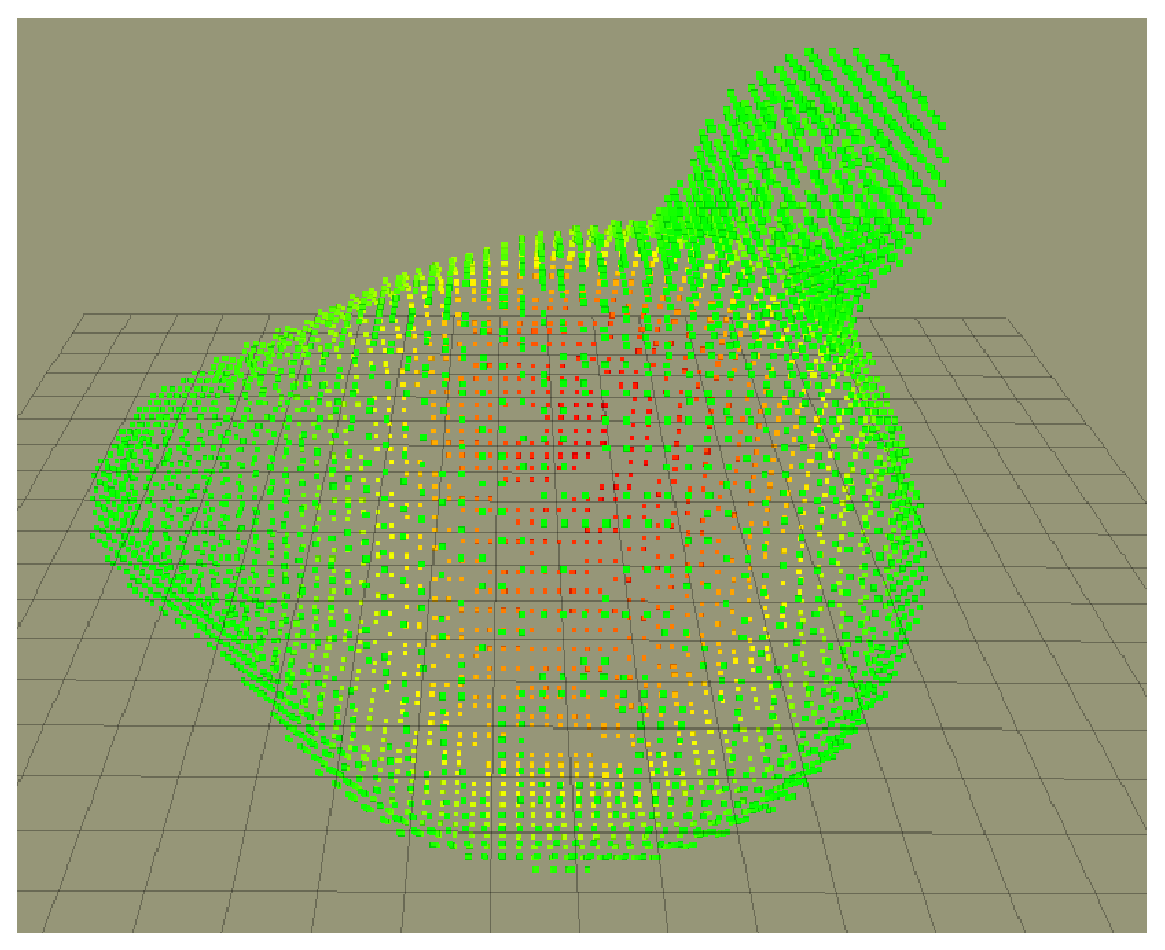
\includegraphics[width=0.45\linewidth]{example.eps}
  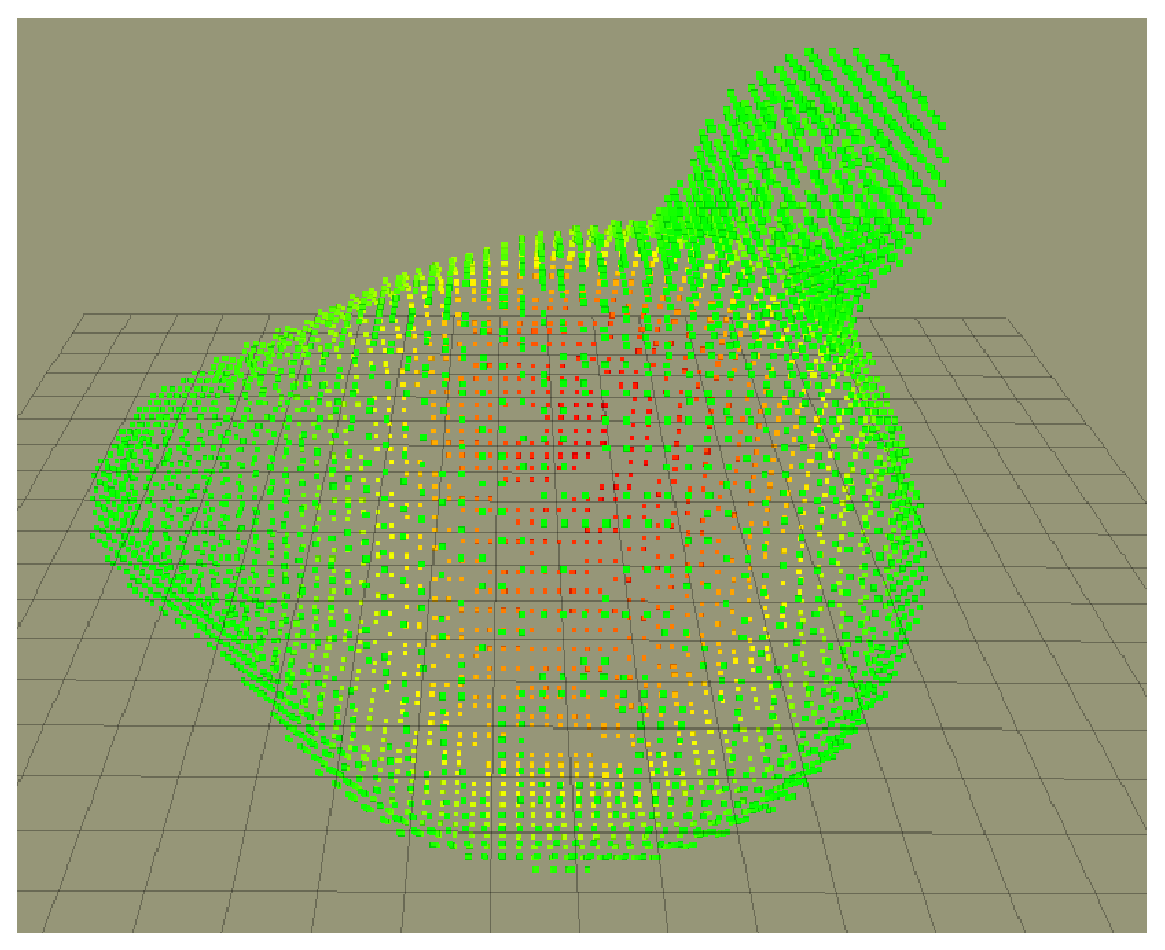
\includegraphics[width=0.45\linewidth]{example.eps}
  }
  \caption{A picture of the in-hand object segmentation using a soft-adaptive hand on a 7-dof arm in the real scene (left) and the resulting point cloud (right).} \label{fig:in-hand-segmentation}
\end{figure}

\begin{algorithm}[h]
\textbf{\textsc{segmenInHand}}$(\mathcal{R}, \kappa, \delta)$\\ %functionname
\LinesNumbered
\DontPrintSemicolon
\SetAlgoVlined \SetKwInOut{Input}{input} \SetKwInOut{Output}{output}
\Input{The point cloud of the scene $\mathcal{P}$, the robot model, $\mathcal{R}$, its visual geometry inflation factor, $\kappa$, and the downsampling resolution, $\delta$.}
\Output{The point cloud of the object isolated from the scene, $\mathcal{O}$.}
  $\mathbf{s} \leftarrow$\textsc{listenToRobotState}($\mathcal{R}$) \\
  $\mathcal{B} \leftarrow$\textsc{computeBoundingBoxes}($\mathcal{R}$, $\mathbf{s}$, $\kappa$) \\
  $\mathcal{O} \leftarrow$\textsc{applyPasstroughFilter}($\mathcal{P}$, $\mathcal{B}$) \\
  $\mathcal{O} \leftarrow$\textsc{applyDownsampleFilter}($\mathcal{O}$, $\delta$) \\
  \Return{$\mathcal{O}$}
\caption{In-hand object segmentation.} \label{alg:in-hand-segmentation}
\end{algorithm}

The \textsc{listenToRobotState}($\cdot$) method considers the measurement of soft-adaptive mechanism

%%%%%%%%%%%%%%%%%%%%%%%%%%%%%%%%%%%%%%%%
\subsection{Shape modelling}
\label{sec:shape}
What makes a good surface representation?
\begin{itemize}
\item Accurate (we handle this with probability)
\item Concise (we might want this)
\item Intuitive specification (we don't need this)
\item Local support
\item Affine invariant 
\item Arbitrary topology (we need this)
\item Guaranteed continuity (we need this)
\item Natural parameterization (we don't need this)
\item Efficient display (we shouldn't need this)
\item Efficient intersections (we could need this)
\end{itemize}

Looks like implicitly defined surfaces are the best...

How do we define implicit function?
\begin{itemize}
\item Algebraics
\item Blobby models
\item Skeletons
\item Procedural
\item Samples
\item Variational
\item Gaussian Process !
\end{itemize}

Variational surfaces:
\begin{itemize}
\item Advantages:
\begin{itemize} 
\item Easy to test if point is on surface
\item Easy to compute intersections/unions/differences
\item Easy to handle topological changes
\end{itemize}
\item Disadvantages:
\begin{itemize}
\item Indirect specification of surface
\item Hard to describe sharp features
\item Hard to enumerate points on surface !
\item Slow rendering !
\end{itemize}
\end{itemize}

Except from rendering and surface explicit related things... but we don't actually need that except from debug.

\begin{figure}
\centering
  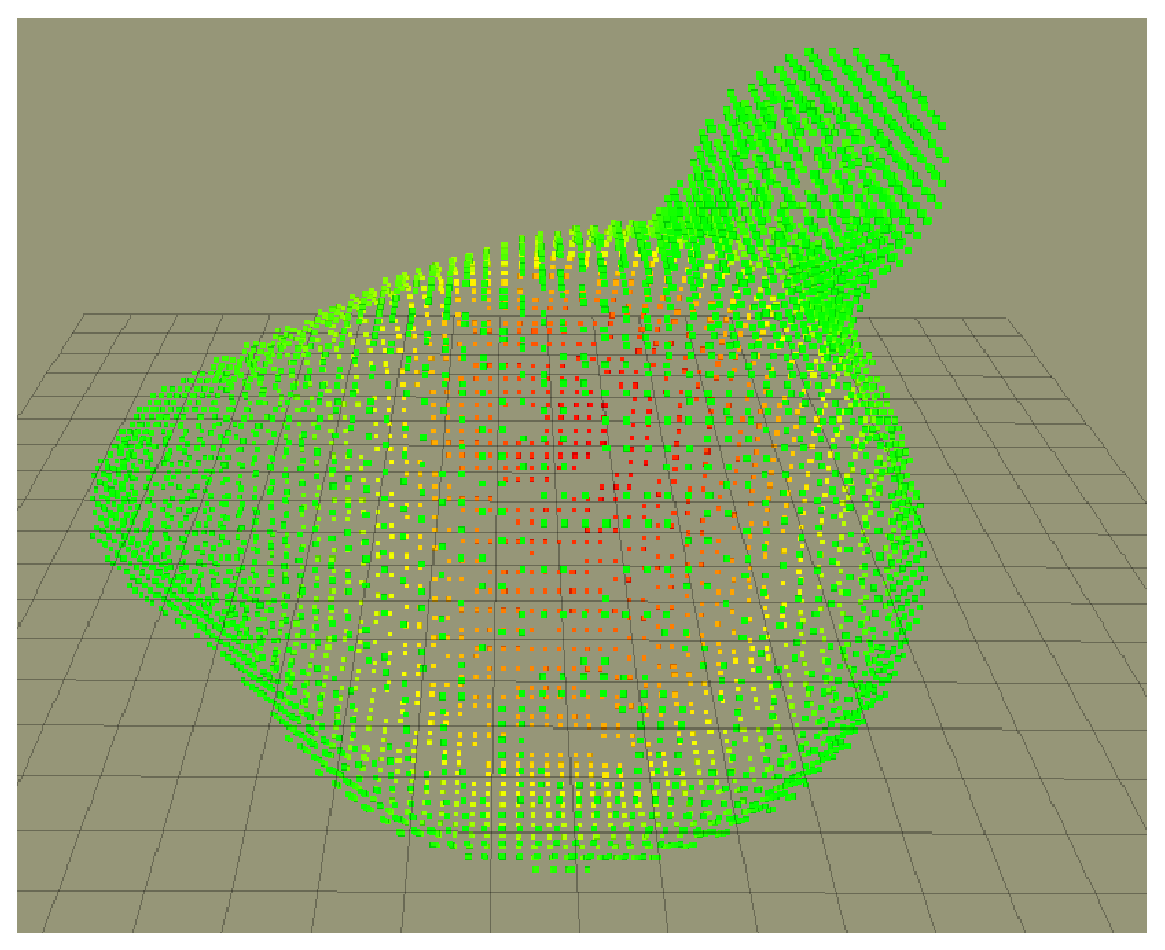
\includegraphics[width=0.9\linewidth]{example.eps}
  \caption{Different shape representations} \label{fig:shape_comparison}
\end{figure}

\begin{algorithm}[h]
\textbf{\textsc{createGaussianProcess}}($X$)\\ %functionname
\LinesNumbered
\DontPrintSemicolon
\SetAlgoVlined \SetKwInOut{Input}{input} \SetKwInOut{Output}{output}
\Input{The training data, $\mathcal{X}$, in the form of a point cloud.}
\Output{The Gaussian Process that models the object shape.}
  $\mathcal{D} \leftarrow$\textsc{deMeanNormalizeAndLabel}(\{$\mathcal{X}$, $\mathbf{0}_{\text{sizeOf}(\mathcal{X})}$\}) \\
  \textsc{addLabeledPoint}(\{$\mathbf{0}_3, -1\}$, $\mathcal{D}$) \\
  \textsc{addLabeledPoints}(\{\textsc{sphere}$(\mathbf{0}_3, 1.1, N)$, $+\mathbf{1}_{N}\}$, $\mathcal{D}$) \\
  $\mathcal{G} \leftarrow$ \textsc{doRegression}($\mathcal{D}$) \\
  \Return $\mathcal{G}$ \\
\caption{Gaussian Process regression} \label{algo:strategy}
\end{algorithm}

%%%%%%%%%%%%%%%%%%%%%%%%%%%%%%%%%%%%%%%%
\subsection{Exploration strategy}
\label{sec:strategy}

We don't need all the conditions described in \citet[Fig.~8]{Jaillet2013Path}.

\begin{algorithm}[h]
\textbf{\textsc{exploreGPAtlasRRT}}$(\mathcal{M}, \mathbb{V}_{max})$\\ %functionname
\LinesNumbered
\DontPrintSemicolon
\SetAlgoVlined \SetKwInOut{Input}{input} \SetKwInOut{Output}{output}
\Input{A Gaussian Process model, $\mathcal{M}$, and the variance threshold, $\mathbb{V}_max$}
\Output{The best next action, $\mathcal{P}$, in the form of a path, if any, or $\varnothing$ otherwise.}
  $\mathcal{P} \leftarrow \emptyset$ \\
  $\mathcal{A} \leftarrow \emptyset$ \textsc{initAtlas}($\mathcal{M}$) \\
  $\mathcal{T} \leftarrow$\textsc{initTrees}($\mathcal{M}$) \\
  $\mathcal{T}_{i} \leftarrow$\textsc{selectTreeToExpand}($\mathcal{T}$, \emph{policy}) \\
  
  $\mathcal{C}_{i,k} \leftarrow$\textsc{generateChart}($\mathbf{x}_{i}$, $\mathcal{M}$) \\
  $X_{i,k} \leftarrow$\textsc{sampleChart}($\mathcal{C}_{i,k}$, $N$) \\
  $\mathbf{x}_{i,k} \leftarrow$\textsc{selectCandidate}($X_{i,k}$) \\
  $\mathbf{x}_{,k} \leftarrow$\textsc{generate}($\mathbf{x}_{i,k}$, $\mathcal{M}$) \\

  \While { $e < h$ }
  {
    $i \leftarrow 0$ \\
    \While{ $i<n$ }
    {
      \Return action 
    }
    $e \leftarrow e + 1$ \\
  }
  \Return{$\varnothing$}

\caption{The best-next tactile action planner} \label{algo:strategy}
\end{algorithm}

A chart, for us, contains the center $\mathbf{x}_c$, such that $\mathbb{E}(\mathcal{S}(\mathbf{x}_c)) \approx 0$, the size $R = \mathbb{V}(\mathcal{S}(\mathbf{x}_c))$ and the gradient information at the center $\frac{\partial \mathcal{S}}{\partial \mathbf{x}} \approx $.

The validity are of each chart is defined as
$\boldsymbol{\Phi}^{T}\boldsymbol{\Phi} \leq \cos(\alpha)$
$\| \mathbf{u}_{j,k} \| \leq \mathbb{V}(\mathcal{x}_{j,k})$

The area covered by a given chart on the surface is never empty, and
it always includes the center of the chart, $\mathbf{x}_{i}$, but its shape depends on the local shape. However, in this work, we are not interested in computing this area, since we will be traversing trees using compliance control to compensate for the errors between linear interpolation between $\mathbf{x}_i$ and $\mathbf{x}_j$ in 3D and actual arbitrary shape countour joinning them.

 A chart is selected at random with uniform distribution
among the all charts in the leafs

%%%%%%%%%%%%%%%%%%%%%%%%%%%%%%%%%%%%%%%%
\subsection{Solution in a nutshell}
\label{sec:summary}

\begin{algorithm}[h]
\textbf{\textsc{ObjectShapeExploration}}$(P, \mathbb{V}_{des})$\\ %functionname
\LinesNumbered
\DontPrintSemicolon
\SetAlgoVlined \SetKwInOut{Input}{input} \SetKwInOut{Output}{output}
\Input{An initial point cloud of the scene, $P$, if any, for instance from visual object segmentation, and the desired variance, $\mathbb{V}_{des}$, for the overall shape estimation.}
\Output{The estimated object shape, $\mathcal{S}$}
  $\mathcal{S} \leftarrow \emptyset$ \\
  \If{ \textsc{isEmpty}$(P)$ }
  {
    $\chi \leftarrow $ \textsc{naiveProbe}() \\
  }
  \Else
  {
    $\chi \leftarrow $ \textsc{segmentObject}($P$) \\
  }
  $\mathcal{S} \leftarrow $\textsc{createGaussianProcess}($\chi$) \\
  \While { \texttt{true} } 
  {
    $\Gamma \leftarrow $\textsc{exploreGPAtlasRRT}$(\mathcal{S}, \mathbb{V}_{des})$ \label{exploration} \\
    \If{ $\Gamma = \emptyset$ }
    {
      \Return {$\mathcal{S}$} \label{solutionfound} \label{end} \\
    }
    \Else
    {
      \textsc{ApproachTo}($\Gamma$) \label{approach} \\
      $\bar{\chi} \leftarrow $\textsc{probeObject}($\Gamma$) \label{probe} \\
      \If{ \textsc{wasContactDetected}() }
      {
        $\upsilon \leftarrow \mathbf{0}_{\text{sizeOf}(\bar{\chi})}$  \label{belonglabel} \\
      }
      \Else
      {
        $\upsilon \leftarrow \mathbf{1}_{\text{sizeOf}(\bar{\chi})}$ \label{nobelonglabel} \\
      }
      \textsc{addLabelPoints}(\{$\bar{\chi}$, $\upsilon$\}, $\chi$) \\
      $\mathcal{S} \leftarrow $\textsc{createGaussianProcess}($\chi$) \\
      \textsc{MoveAway}() \label{away} \\
    }
  }
\caption{Proposed object shape modelling} \label{alg:strategy}
\end{algorithm}

In the \textsc{ApproachTo}(line~\ref{approach}) (\textsc{MoveAway})(line~\ref{away}) phase, the robot uses position control and standard motion planning techniques with collision avoidance. Since we are modelling the shape, we need to ensure that everytime the robot moves close (away) from the object, it does not collide with the object. It is tentative to use the current estimated shape, but since we are not actually computing it explicitly in our approach, we choose the bounding sphere as the collision geometry of the object. Thus the robot moves towards (away from) the surface at the contact location in the normal direction until reaching the bounding sphere. After that, a standard motion planning is used to approach the object (get to the rest position).

In the \textsc{probeObject}(\ref{probe}) phase, the robot is within the bounding sphere and uses Cartesian impedance control, with the Cartesian force, pose and impedance set properly for the given setup. These implementation details are given in the next section. Since we don't actually know where the surface is, we need to whether the robot actually touched something or not, in order to properly label the acquisition (lines~\ref{belonglabel} and~\ref{nobelonglabel}) 

The method finishes when the method \textsc{exploreGPAtlasRRT}(line~\ref{exploration}) described in Algorithm~\ref{algo:strategy} has explore sufficiently the estimated shape and could not find an exploratory action $\Gamma$ (line~\ref{end}), i.e. the object shape is probabilistically estimated within the 95\% of the confidence interval computed from $\mathbb{V}_{des}$. 

The complete solution of the problem as stated in~\ref{sec:scope} is depicted in Algorithm~\ref{alg:strategy}.

\subsection{Parameters  and probabilistic completeness}
\label{sec:analsys}

We can safely assume that the surface has only one component when seen as a manifold.
